% Based on https://github.com/JavierGelatti/Formato-LaTeX-CoNaIISI
% Overleaf Project https://www.overleaf.com/project/64cdfd2c62d20c8819796f78

\documentclass[12pt,a4paper,final,oneside,notitlepage]{article}
\usepackage[utf8]{inputenc} % Acentos, etc
\usepackage[spanish]{babel} % Idioma
\usepackage[left=2.5cm,right=2.5cm,top=2.5cm,bottom=2.5cm]{geometry} % Margenes
\usepackage[justification=centering,margin=.3cm]{caption} % Epígrafes

\usepackage{mathptmx} % Times New Roman
\usepackage{amsmath}
\usepackage{amsfonts}
\usepackage{amssymb}
\usepackage{titlesec}
\usepackage{multicol} % Dos columnas
\setlength\columnsep{1cm}

\usepackage[hidelinks]{hyperref} % Hipervinculos en color negro

\usepackage{enumitem}
\usepackage{xcolor}
\usepackage{graphicx}
\usepackage{tikz}
% \usepackage[font=small, justification=justified, format=plain]{caption} % Para las captions por si hay errores
\usepackage{graphicx}

\usepackage{setspace}
\usepackage{titlesec} % Formato de titulos de secciones

\titleformat{\section}{\bfseries\normalsize}{}{0pt}{}
\titlespacing*{\section}{0pt}{1em}{0pt}

\titleformat{\subsection}{\bfseries\normalsize}{}{}{}
\titleformat{\subsubsection}{\bfseries\normalsize}{\quad}{}{}

\pagestyle{empty} % Sin número de página

\setlength{\parindent}{0cm}
\setlength{\parskip}{0em}

\makeatletter

% Metadatos
\def\email#1{\gdef\@email{#1}}
\def\@email{\@latex@warning@no@line{No \noexpand\email given}}

\def\universidad#1{\gdef\@universidad{#1}}
\def\@universidad{\@latex@warning@no@line{No \noexpand\universidad given}}

% Título
\newcommand{\titulo} {
	\begin{center}
		{\LARGE\bfseries\@title}
		
		\vspace{2em}
		{\Large\bfseries\@author}
		\vspace{.5em}
		
		{\normalsize\bfseries\itshape\@universidad}
		\vspace{2em}
	\end{center}
}
\makeatother

% Minisección (para las palabras clave, agradecimientos, etc)
\newcommand{\miniseccion}[1] {
 	\vspace{0.5em}
	{\footnotesize\ignorespaces\textbf{#1} \par}
	\ignorespaces
}

% \titlespacing*{\minisection}{0pt}{0.5em}{0pt}
% Abstract
\newcommand{\resumen}[1] {
	\miniseccion{Abstract}
	{\noindent\footnotesize\textit{#1} \par}
}

% Figuras
\newenvironment{Figure}
  {\par\medskip\noindent\minipage{\linewidth}}
  {\endminipage\par\medskip}
 
\newcommand{\bibliofont}{\footnotesize}

\let\OLDthebibliography\thebibliography
\renewcommand\thebibliography[1]{
  \OLDthebibliography{#1}
  \bibliofont
  \setlength{\parskip}{0pt}
  \setlength{\itemsep}{0pt plus 0.2ex}
  }
  
  
\graphicspath{ {./img/} }

% \author{Oscar Ricardo Bruno}
\title{Repositorio descentralizado para la gestión y el aprendizaje de algoritmos de speedcubing}
% \email{skielcast@gmail.com}
% \universidad{Universidad Tecnológica Nacional, Facultad Regional Buenos Aires}

\begin{document}
\titulo

\begin{multicols}{2}

\resumen{
El presente documento narrará en profundidad el desarrollo de un sistema totalmente descentralizado construido para suplir la necesidad de la existencia de un repositorio de algoritmos de speedcubing \footnote{El speedcubing es el deporte de resolver cubos de Rubik o puzzles similares en el menor tiempo posible. Quienes lo practican se conocen como ``speedcubers''.} que pueda ser mantenido por la propia comunidad que lo utiliza y no por una entidad única. De la misma forma que los ajedrecistas estudian aperturas, los speedcubers estudian algoritmos para resolver cubos de Rubik de formas más rápidas.
}

\miniseccion{Palabras Clave}

{\footnotesize
descentralización, blockchain, web3, speedcubing, cubo de rubik
\par}

\section{Introducción}

El sistema desarrollado se encuentra estrictamente ligado a una problemática presente en el mundo del speedcubing. De la misma manera que un ajedrecista necesita estudiar aperturas, analizarlas, y practicarlas, un speedcuber necesita aprender los denominados ``algoritmos''.\\

Se denomina de esta forma en el speedcubing a una secuencia de movimientos que, al aplicarse en un puzzle, afectan a las piezas del mismo de una forma previamente conocida. Es decir, un algoritmo se utiliza para resolver problemas comunes de manera óptima, previa memorización del mismo.\\

Hasta el desarrollo de este trabajo, no existía ningún tipo de sistema o plataforma que reuniera todos los algoritmos utilizados por los métodos más comunes en un mismo lugar, donde además se pudiera practicarlos siguiendo el progreso personal, y no se dependiera de una única persona o entidad para mantenerlo.
En reiteradas ocasiones existieron proyectos similares, pero al siempre depender de una única persona resultaron insostenibles en el tiempo y la comunidad de speedcubing se encontró migrando una y otra vez de plataforma.\\

Se busca que \textit{Cubitorium}\footnote{Nombre comercial del sistema.} sea la alternativa final para los speedcubers en este sentido. Para proveer descentralización y trasladar el mantenimiento del sistema a la comunidad misma se desarrolló un back-end hosteado en la blockchain de Solana\cite{solana}, y un front-end desplegado utilizando la tecnología de IPFS\cite{ipfs}.\\

En este documento se narrará en detalle la naturaleza de un algoritmo de speedcubing, así como la implementación paso a paso de cómo se ha modelado un cubo de Rubik programáticamente para poder aplicar secuencias de movimientos y validar que funcionen correctamente, y la arquitectura del sistema en cuestión.

\section{Speedcubing}

Se narrará primeramente el funcionamiento de un método de speedcubing a grandes rasgos, y el uso esperado de este sistema por parte de un speedcuber.\\

En este deporte, cada puzzle se resuelve de acuerdo a un método que divide el problema total en distintas etapas o sub-problemas. Algunas de ellas, generalmente las iniciales, se pueden completar de forma intuitiva. Sin embargo, al avanzar en la resolución, el rompecabezas se restringe hasta llegar a un punto en el que es extremadamente difícil deducir soluciones en un tiempo muy corto. Por esta razón, las últimas etapas de los métodos de speedcubing consisten en aplicar un algoritmo que resuelva el caso que se presenta.\\

Si un método tiene una última etapa con 22 casos posibles\footnote{La última etapa del método más popular para el cubo de Rubik, ``PLL'', tiene 22 casos posibles incluyendo el estado resuelto.}, entonces un speedcuber memorizará y practicará todos estos casos para poder resolver cualquier estado que se le presente al llegar a esta etapa en tan solo segundos.\\

De este modo, una vista del sistema podría verse como sigue:\\

\begin{Figure}
\centering
    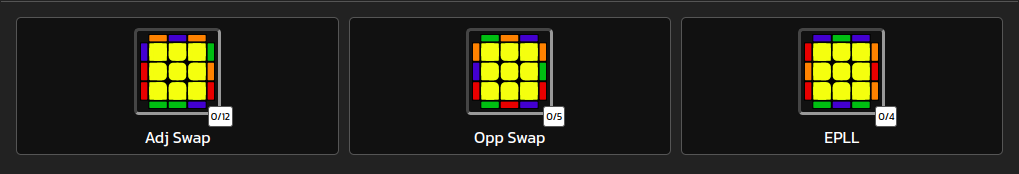
\includegraphics[width=0.9\textwidth]{img/plls_speedcubedb.png}
 \captionof{figure}{Vista de etapa ``PLL'' en SpeedcubeDB\cite{speedcubedb}}
 \label{fig:pll-speedcubedb}
\end{Figure}

\begin{Figure}
\centering
    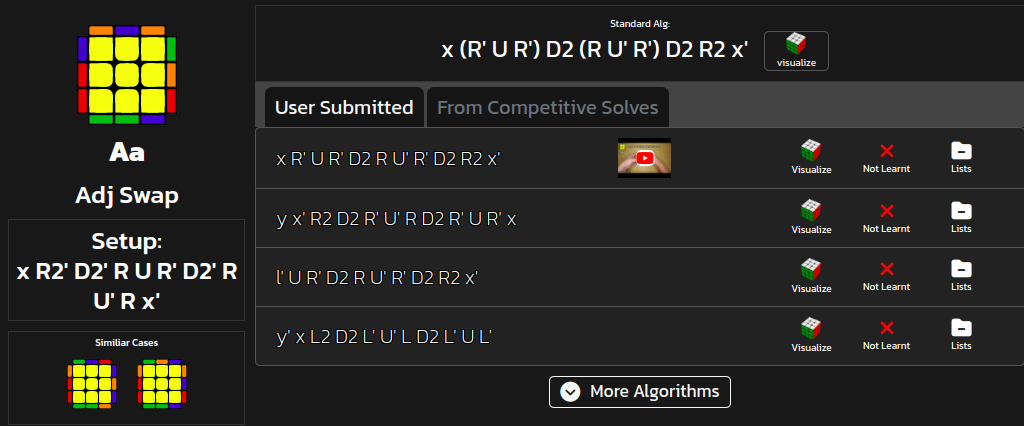
\includegraphics[width=0.9\textwidth]{img/aperm-speedcubedb.png}
 \captionof{figure}{Vista de algoritmo puntual en SpeedcubeDB\cite{speedcubedb}}
 \label{fig:aperm-speedcubedb}
\end{Figure}

Allí, un usuario podría elegir una serie de algoritmos del ``catálogo'' y en base a eso leerlos, aprenderlos, y practicarlos.

Los algoritmos no son únicos. Es decir, para cada caso existen varias formas (de hecho, infinitas) de resolverlo. Sin embargo, solo algunas de estas soluciones son viables para el speedcubing. Muchas de ellas son igualmente buenas, y la preferencia sobre una u otra es una cuestión meramente personal.
En algunos casos, incluso, sucede que un speedcuber descubre una nueva forma de resolver un caso y causa que sea la nueva opción preferida.

\section{Modelo matemático}

Dada la realidad enunciada en la sección anterior, nuestro sistema admite la carga de algoritmos nuevos. Al carecer de usuarios privilegiados\footnote{El sistema cuenta con usuarios administradores, pero no se espera que formen parte de los casos de uso típicos del mismo. Es decir, estos usuarios solamente se encargarían de definir configuraciones globales del entorno por única vez o muy rara vez.}, la única manera de validar que el algoritmo ingresado sea correcto es implementando un modelo matemático del cubo de Rubik que permita validar las soluciones automáticamente. Narraremos a continuación cómo se ha conseguido hacer eso exitosamente.\\

Un cubo de Rubik puede modelarse muy sencillamente como dos arreglos de un tipo abstracto. Al tener un cubo 12 aristas y 8 esquinas\footnote{En la jerga del speedcubing se denomina ``esquina'' a un vértice del cubo.}, bastaría con modelar dos tipos de elementos y contar con 12 y 8 instancias de cada uno respectivamente. En pseudocódigo:

\begin{verbatim}
    pieza {
        id: T,
        orientacion: u8
    }

    esquinas: [pieza; 8]
    aristas: [pieza; 12]
\end{verbatim}

En esta representación, llamamos ``\textit{id}'' a un identificador unívoco para cada pieza. Por ejemplo, podría tratarse de los colores que la componen, o un número arbitrario de referencia.
Por otro lado, llamamos ``\textit{orientación}'' a la dirección en la que se encuentre esta pieza. Debido a que las esquinas tienen 3 lados y las aristas 2, puede suceder que se encuentren en la misma posición pero con una orientación diferente.\\

Dada la posición relativa de cada elemento dentro de su arreglo, podremos determinar su permutación. Dado el valor que contenga, podremos determinar su orientación.\\

Esta representación es una de las posibles, y la usaremos de base para modelar el cubo de Rubik en el back-end de Solana programado en Rust\cite{rust}.\\

En nuestro sistema, en lugar de contar con arreglos de una estructura, decidimos separarlo en cuatro arreglos por mera conveniencia: uno para la orientación y uno para la permutación de cada tipo de pieza, dando 4 en total:

\begin{verbatim}
    struct Cube {
        co: [u8; 8],
        cp: [u8; 8],
        eo: [u8; 12],
        ep: [u8; 12],
    }
\end{verbatim}

Estos arreglos funcionarán como dos grupos de dos, siendo que la permutación de los elementos se correspondan a aquellos arreglos modelando tipos distintos de piezas debe ser modificada siempre de la misma forma.\\

Usaremos los prefijos ``o'' y ``p'' para referirnos a la orientación y permutación, y los sufijos ``c'' y ``e'' para referirnos a las esquinas (\textit{corners}) y aristas (\textit{edges}).\\

Como identificadores, utilizaremos números enteros. Es decir, \texttt{[1,4,2,3,6,5,8,7]} podría representar una permutación válida de las esquinas (\texttt{cp}), mientras que \texttt{[1,2,3,4,5,6,7,8]} representaría el estado resuelto.\\

Para la orientación, definiremos de forma arbitraria valores para cada tipo de pieza según su característica. Esto significa valores posibles de \texttt{0, 1 y 2} para las esquinas (al tener 3 lados), y de \texttt{0 y 1} para las aristas por la misma razón. Definiremos la orientación de las esquinas como se muestra, según la ubicación del ``sticker'' blanco o amarillo de cada una:

\begin{Figure}
\centering
    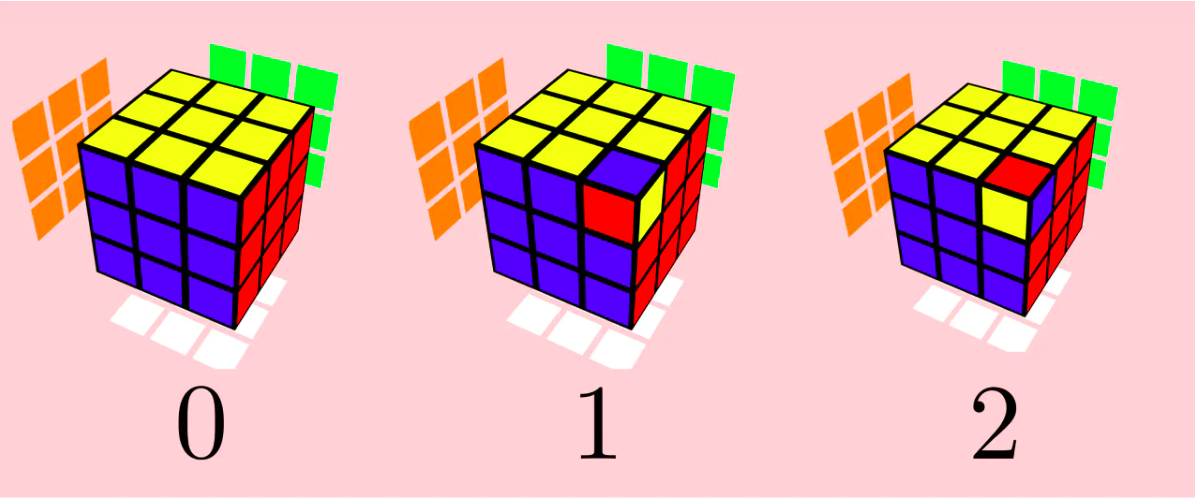
\includegraphics[width=0.9\textwidth]{img/rotations.png}
 \captionof{figure}{Definición de la orientación de esquinas}
 \label{fig:rotations}
\end{Figure}

De forma similar, definiremos la orientación de las aristas como una propiedad intrínseca de cada pieza que cambia de valor cada vez que esa pieza está presente en la cara frontal o trasera y esa misma cara realiza un giro simple.\footnote{Esta decisión es arbitraria en cuanto al eje, pero tiene una explicación matemática por detrás relacionada a la teoría de grupos. Consideramos que excede el objetivo de este documento, por lo que no se desarrollará su naturaleza.} Con esto en mente, \texttt{[0,1,1,0,0,1,1,0,0,1,1,0]} podría ser un arreglo de orientaciones de aristas válido (\texttt{eo}), y \texttt{[0,0,0,0,0,0,0,0,0,0,0,0,0]} el estado inicial del mismo.\\

Dadas estas definiciones, podremos construir un cubo de Rubik resuelto como sigue:

\begin{verbatim}
    let cube: Cube = Cube {
       cp: Vec::from_iter(1..=8),
       co: vec![0; 8],
       ep: Vec::from_iter(1..=12),
       eo: vec![0; 12],
    };
\end{verbatim}

Finalmente, solo restará definir cómo modifica cada giro aplicado en el mismo a estos arreglos, y con esto podremos aplicar movimientos en nuestro cubo de Rubik modelado matemáticamente.

\section{Arquitectura del sistema y tecnologías}

Esta lógica se implementa en Rust\cite{rust}, en un programa de Solana\cite{solana} desarrollado bajo el framework de Anchor\cite{anchor}. El código fuente aún no ha sido publicado al momento de la redacción de este documento.\\

Al contar con un programa de Solana, se resuelven dos componentes principales del sistema: el procesamiento en back-end y la persistencia. La blockchain de Solana hace las veces de ambos componentes:

\begin{itemize}
    \item \textbf{Persistencia:} Solana es una blockchain con alta capacidad de persistencia escalable. Cada programa puede reservar dinámicamente el almacenamiento que precise y persistir allí los datos de manera indefinida.\footnote{El almacenamiento tiene un costo proporcional a los bytes almacenados, pero este costo es muy bajo (0.00089784 SOL por byte al momento de escribir este documento, cerca de 2 centavos de dólar).}
    \item \textbf{Procesamiento:} Los programas en Solana existen con el propósito de realizar cálculos de manera descentralizada. Este componente reemplaza lo que, de haber implementado este sistema de forma tradicional, podría haber sido un módulo de \textit{cloud computing}. Solana permite un \textit{throughput} de 65000 transacciones por segundo\cite{solana-throughput}.
\end{itemize}

Descentralizar esta parte del sistema de esta manera nos permite desentendernos de los principales factores que funcionaban como dolor en los otros sistemas que buscaron resolver la problemática que atacamos. Por un lado, una vez desplegado el programa en Solana ya no hay que encargarse de realizar pagos periódicos o de ningún tipo para mantenerlo en funcionamiento. Por el otro, nadie podrá darlo de baja una vez sea publicado.\\

Seguirá existiendo la necesidad de fondear el sistema esporádicamente, ya que aumentar el espacio de almacenamiento\footnote{Precisamente, cada \textit{alloc} de \textit{Program Derived Accounts}.} implica tener que pagar por cada byte adicional, y esta responsabilidad fue trasladada al programa que será fondeado inicialmente. Será en el futuro la misma comunidad de speedcubing la encargada de transferir dinero a la cuenta del programa.\footnote{La cuenta donde se almacenan las criptomonedas no tiene custodia; es decir, la única forma de usar ese dinero es mediante la lógica misma que está redactada en ese programa. Una vez enviada ahí, nadie puede usarla para ningún otro propósito que no esté escrito en su código.}\\

Existe una capa intermedia entre el back-end (programa blockchain) y el front-end: el SDK. Este módulo, materializado como una clase de TypeScript\cite{ts} provee encapsulamiento de todas las funcionalidades englobadas por el programa.\\

Ya que los programas en Solana solo admiten comunicaciones en formato serializado, es necesario abstraer este comportamiento. La estructura de un llamado a un programa en Solana es la siguiente:

\begin{verbatim}
    struct ProgramCall {
        program_id: Pubkey,
        data: &[u8],
        accounts: &[AccountInfo],
    }
\end{verbatim}

En donde \textit{\texttt{program\_id}} es la dirección o identificador del programa, \textit{\texttt{data}} es el payload serializado\footnote{En Rust, \texttt{\&[u8]} es comparable a un \texttt{void*} en C.}, y \textit{\texttt{accounts}} es un arreglo de las cuentas de contexto que utilizará la instrucción\footnote{Resumidamente, las direcciones de memoria solo lectura y modo escritura que accederá una función durante su ejecución.}.\\

Por lo tanto, todo llamado al programa debe contener un indicador que referencie a qué función llamar, seguido de eventuales argumentos. Es precisamente esto uno de los problemas que el framework Anchor\cite{anchor} nos resuelve. Anchor asigna a cada función (denominadas ``instrucciones'') un hash unívoco\footnote{Primeros 8 bytes del hash SHA256 de la cadena \texttt{``global:x''} siendo \texttt{x} el nombre de la instrucción.}, y luego serializa según el estándar de \textit{\texttt{borsh}}\cite{borsh} los parámetros enviados.\\

Aún así, si bien esto se materializa como un cliente de Typescript provisto por Anchor, no es suficiente para utilizar desde un front-end. Sucede que el tercer argumento, \textit{\texttt{accounts}}, no siempre se completa de forma trivial\footnote{Resumidamente, algunas direcciones de memoria se deben calcular o averiguar realizando consultas de antemano en Solana.}. Es por esto que mediante una clase personalizada es posible encapsular la lógica necesaria para llenar este campo y abstraer al desarrollador front-end de las particularidades de la blockchain de Solana a la hora de integrar su desarrollo con el módulo de back-end provisto.\\

Finalmente, el sistema tiene una interfaz gráfica para el usuario desarrollada en React\cite{react}. Este módulo interactúa de forma directa con el SDK descripto anteriormente, quien a su vez se comunica directamente con la blockchain de Solana. Para dar completitud a la descentralización del sistema, todo el front-end se despliega en el sistema de IPFS\cite{ipfs}.\\

IPFS es un filesystem distribuido que direcciona los archivos en base a su contenido, en lugar de en base a su dirección como lo hace la web tradicional. Los archivos subidos a este sistema serán replicados en los nodos de la red y, al momento en el que un usuario desee acceder al archivo, será accedido del nodo más cercano de una forma similar a la que un sistema \textit{torrent} lo consigue.\\

Los nodos de IPFS son ligeros y sencillos de levantar\footnote{De hecho, el navegador Brave funciona como un nodo de IPFS\cite{brave-ipfs}.}, pero también son sencillos de dar de baja. Si el archivo en cuestión no fue transmitido lo suficiente, desaparecerá por siempre de la red. Para mitigar este problema, existen servicios de ``pinning'' que activamente mantienen vivo un archivo con el fin de que no desaparezca de la red.\\

Un archivo accedido frecuentemente por una comunidad entera globalizada difícilmente será eliminado de la red, ya que éste será replicado en numerosos nodos distribuidos de una manera geográficamente diversa.\\

\begin{Figure}
\centering
    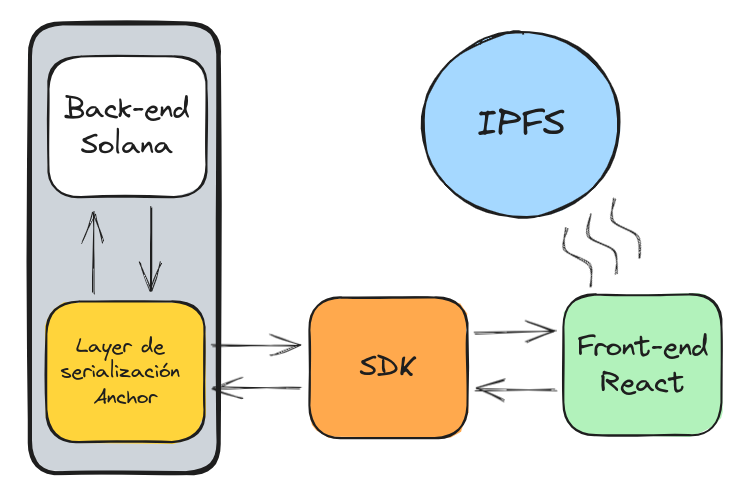
\includegraphics[width=0.75\textwidth]{img/cubitorium_arch.png}
 \captionof{figure}{Arquitectura del sistema}
 \label{fig:arquitectura}
\end{Figure}

\section{Conclusión y Trabajos Futuros}

Se concluye la importancia de la independencia de una comunidad como grupo. Siendo un conjunto muy grande, diverso y distribuido de personas con un interés en común, es menester ser capaz de entregar la custodia y responsabilidad de mantenimiento de los servicios utilizados a la misma comunidad, sin depender de una parte externa.\\

En el pasado la comunidad de speedcubing ha sufrido muchos inconvenientes por el hecho de no contar con un repositorio de algoritmos descentralizado, siendo el último de estos retrocesos este mismo año, en el que SpeedcubeDB ha sido dado de bajas numerosas veces.\\

La tecnología de la era que vivimos ya nos entrega la capacidad de construir sistemas con paradigmas totalmente diferentes a lo habitual, a modo de empoderar a un grupo de personas a través de la lógica de un programa y no depender simplemente de la confianza y la buena voluntad de partes desconocidas.\\

Como trabajos futuros se proponen extensiones de \textit{Cubitorium} para almacenar otro tipo de informaciones útiles para speedcubers, como reconstrucciones o distintos métodos, a la par de que se busca incentivar el desarrollo de nuevos sistemas descentralizados en contextos en los cuales sean una solución apropiada, más allá del speedcubing.

%\IEEEtriggeratref{8}
% The "triggered" command can be changed if desired:
%\IEEEtriggercmd{\enlargethispage{-5in}}

\begin{thebibliography}{99}

\bibitem{solana}
Blockchain de Solana. \url{https://solana.com/}.

\bibitem{ipfs}
InterPlanetary File System. \url{https://ipfs.tech/}.

\bibitem{speedcubedb}
SpeedcubeDB. Repositorio similar a Cubitorium que será descontinuado pronto. \url{https://speedcubedb.com/}.

\bibitem{rust}
Lenguaje Rust. \url{https://www.rust-lang.org/}.

\bibitem{anchor}
Anchor, framework de desarrollo de programas de Solana. \url{https://www.anchor-lang.com/}.

\bibitem{solana-throughput}
Estudio del rendimiento de Solana en octubre del 2022. \url{https://solana.com/news/network-performance-report-october-2022}.

\bibitem{react}
React, librería para desarrollo front-end. \url{https://react.dev/}.

\bibitem{ts}
Lenguaje Typescript. \url{https://www.typescriptlang.org/}.

\bibitem{borsh}
Borsh: Binary Object Representation Serializer for Hashing. \url{https://borsh.io/}.

\bibitem{brave-ipfs}
Soporte de IPFS en navegador Brave. \url{https://brave.com/ipfs-support/}.

\end{thebibliography}

% \miniseccion{Datos de Contacto}

% {\it\footnotesize

% Agustín Villarreal - agustinvilla@frba.utn.edu.ar\\
% Cristóbal Szkutnik - cszkutnik@frba.utn.edu.ar\\
% Guido Dipietro - gdipietro@frba.utn.edu.ar\\
% Guido Enrique - genriquezabala@frba.utn.edu.ar\\
% Matías Davicino - mdavicino@frba.utn.edu.ar\\

% \par}

\end{multicols}

\end{document}